\section{Windowed least-squares framework}\label{sec:tclspg} 
This section
outlines the proposed \methodNameLower\ 
(\methodAcronym) framework. In contrast to (1) Galerkin projection, 
which minimizes (time-continuous) FOM ODE residual at a time instance, 
(2) LSPG projection, 
which minimizes
the (time-discrete) FOM O$\Delta$E residual 
over a time step, and (3) ST-LSPG projection, 
which minimizes
the  FOM O$\Delta$E residual 
over the entire time interval, the proposed \methodAcronym\ method sequentially minimizes the 
time-continuous FOM ODE residual over a series of arbitrarily defined
\textit{time windows}. The formulation is compatible with both \spatialAcronym\ and \spaceTimeAcronym\ trial subspaces. 
In this section, we start by outlining the \methodAcronym\ formulation  
for a general space--time trial subspace. We then examine the \spatialAcronym\ 
trial subspace, followed by the \spaceTimeAcronym\ trial subspace. In each case, we derive the stationary conditions 
associated with the associated residual-minimization problems.
 %The proposed method can be formulated equivalently from
%two viewpoints. The first formulation corresponds to a sequence of
%minimization problems for the generalized coordinates that minimize the FOM
%ODE residual over each time slab. We refer to this as the 
%\textit{residual-minimization viewpoint}. The second viewpoint corresponds to
%formulating an optimal control problem for the Galerkin ROM. In this
%viewpoint, the \methodAcronym\ method is formulated as an optimal control
%problem in where the objective is to find a ``controller" that minimizes the
%residual of the Galerkin ROM. We refer to this viewpoint as the
%\textit{optimal control viewpoint.}  This section outlines the derivation of the \methodAcronym\ method
%from both the residual minimization and optimal control viewpoints.

%\subsection{Formulation of the Time-Continuous LSPG Method} In contrast to
%the LSPG approach, which minimizes the fully discrete residual over a
%time-step, the present work proposes minimizing the time-continuous FOM ODE
%residual over time slabs. The proposed method can be formulated equivalently
%from two viewpoints. The first approach formulates the problem from a
%standard calculus of variations viewpoint and is analogous to the classic
%residual minimization process used in the LSPG method (but here performed at
%the continuous level). The second viewpoint corresponds to formulating an
%optimal control problem in Lagrange form (which is a specific instance of an
%optimal control problem of Bolza type). In this viewpoint, the
%\methodAcronym\ is formulated as an optimal control problem in where the
%objective is to find a ``controller" that minimizes the residual of the
%Galerkin ROM. We now outline both of these (equivalent) formulations. 
%
\subsection{Windowed least-squares for general space--time trial subspaces} 
We begin by introducing a (nonuniform) partition of the time domain $[0,T]$
into $\nslabs$ non-overlapping windows $[\timeStartArg{n} ,
\timeEndArg{n}]\subseteq[0,T]$ of length $\DeltaSlabArg{n}\defeq\timeEndArg{n} -
\timeStartArg{n}$, $n=1,\ldots,\nslabs$ such that 
$\timeStartArg{1} = 0$, $\timeEndArg{\nslabs} = T$, and
$\timeStartArg{n+1} = \timeEndArg{n}$,
$n=1,\ldots,\nslabs-1$; Fig.~\ref{fig:slab_fig} depicts this partitioning.
\begin{figure} 
\begin{centering} 
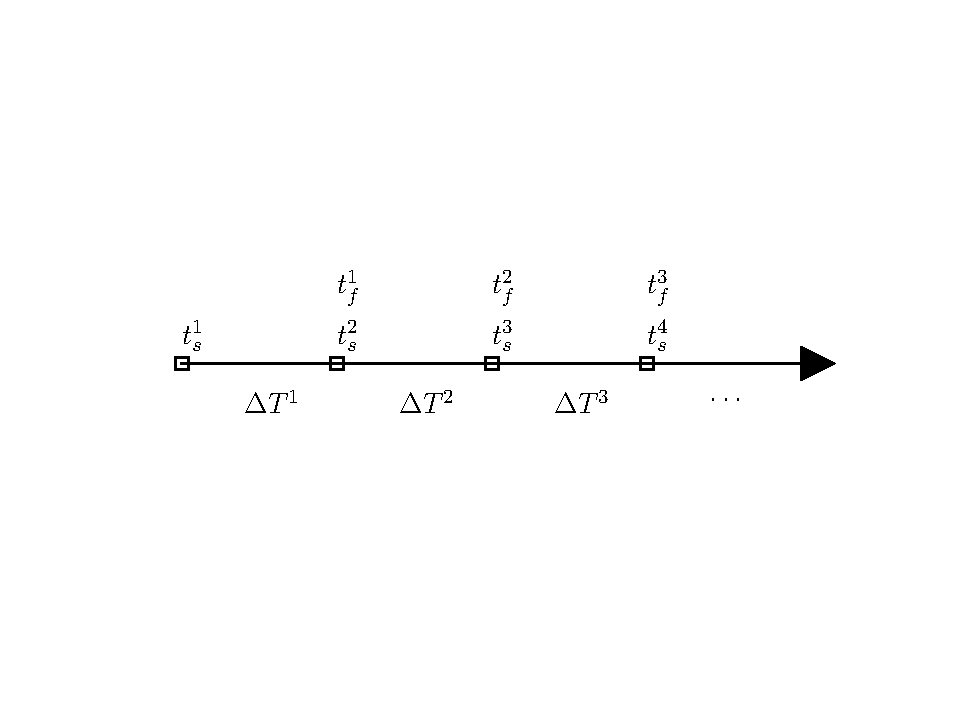
\includegraphics[trim={0.0cm 5cm 0cm 3cm},clip,width=1.0\textwidth]{figs/time_grid.pdf} \caption{Decomposition of time
domain into time windows.} \label{fig:slab_fig} \end{centering} 
\end{figure}
Over the $n$th time window, we approximate the FOM ODE solution as 
$\approxstate^n(t)\approx \stateFOM(t)$,
$t\in[\timeStartArg{n},\timeEndArg{n}]$, which is enforced to reside in 
the $n$th space--time trial subspace such that
\begin{equation}
\approxstate^n \in \stspace^n \subseteq \RR{N} \otimes \timeSpaceArg{n} , \qquad  n = 1,\ldots,\nslabs,
\end{equation}
where $\timeSpaceArg{n}$ denotes the set of real-valued functions acting on
$[\timeStartArg{n},\timeEndArg{n}]$ (i.e., $\timeSpaceArg{n} = \{f\,|\,f:[\timeStartArg{n},\timeEndArg{n}]\rightarrow\RR{}\}$)
and
$\approxstate^n \in\RR{\fomdim}\otimes\timeSpaceArg{n}$. 

\KTC{HERE}
Over the $n$th window, define the objective functional
\begin{equation}\label{eq:obj}
\begin{split} \mathcal{J}^n &\vcentcolon \statey \mapsto
\frac{1}{2} \int_{\timeStartArg{n}}^{\timeEndArg{n}} \big[ \dot{\statey}(t)
- \velocity(\stateyArg{}{t},t) \big]^T \stweightingMatArgt{n}{t} \big[
\dot{\statey}(t) - \velocity(\stateyArg{}{t},t) \big] d t \\
%&\vcentcolon \RR{\fomdim} \times [\timeStartArg{n},\timeEndArg{n}] \rightarrow
%\RR{}, \end{align}
&\vcentcolon \RR{\fomdim}\otimes \timeSpaceArg{n}  \rightarrow
\RR{}_+, 
\end{split}
\end{equation}
%\begin{align}\label{eq:obj} \mathcal{J}^n &\vcentcolon \state \mapsto
%\frac{1}{2} \int_{\timeStartArg{n}}^{\timeEndArg{n}} \resid(\state)^T
%\stweightingMat \resid(\state) d\tau \\ &\vcentcolon \RR{\fomdim} \times
%[0,T] \rightarrow \RR{}.  \end{align}
where $\stweightingMatArg{n} \equiv \stweightingMatOneArg{ }^T
\stweightingMatOneArg{ } \in \RR{\fomdim \times \fomdim}$ denotes a
symmetric positive semi-definite matrix that can enable hyper-reduction, for
example. For notational simplicity, 
we employ the same weighting matrix for all time windows. 

The \methodAcronym\ framework sequentially computes approximate solutions
$\approxstateArgnt{n}\in\stspace^n$, $n=1,\ldots,\nslabs$, where 
$\approxstateArgnt{n}$ is the solution to the
minimization problem
\begin{equation}\label{eq:tclsrm}
\begin{split}
      &\underset{\statey \in \stspace^n}{\text{minimize}} \; \mathcal{J}^n(\statey), \\
			&\text{subject to } \;  \statey(\timeStartArg{n}) =
\begin{cases}\mathbb{P}^n (\approxstateArgnt{n-1})(\timeEndArg{n-1}) & n = 2,\ldots,\nslabs \\
\mathbb{P}^n( \stateFOMArgnt{1})(0)& n=1, \end{cases} 
\end{split}
\end{equation}
%\methodAcronym\ computes a sequence of approximate solutions $\approxstateArgnt{n}$ as the solution to the minimization problem,
%\begin{equation}\label{eq:tclsrm}
%\begin{split}
%       &\approxstateArgnt{n} =  \underset{\statey \in \stspace^n}{\text{arg\,min}} \; \mathcal{J}^n(\statey), \\ 
%      &\text{subject to }\;  \approxstateArg{n}{\timeStartArg{n}} =
%\begin{cases}\mathbb{P}^n (\approxstateArgnt{n-1})(\timeEndArg{n-1}) & n = 2,\ldots,\nslabs \\
%\mathbb{P}^n( \stateFOMArgnt{1})(0)& n=1, \end{cases} 
%\end{split}
%\end{equation}
where $\mathbb{P}^n: \RR{N} \otimes \timeSpaceArg{n} \rightarrow \stspaceArg{n}$ is an orthogonal projection onto the 
trial subspace (e.g., $\elltwo$).
%\methodAcronym\ generates approximations to~\eqref{eq:FOM} by sequentially minimizing
%the FOM ODE residual over the trial space for each time slab.
%\methodAcronym\ is defined as follows,
%\begin{equation}\label{eq:tclsrm}
%\approxstate^n= \underset{\statey \in \stspace^n}{\text{arg\,min } }
%\mathcal{J}^n(\statey), \qquad n = 1,2,...,\nslabs,
%\end{equation}
% subject to
%the boundary condition, \begin{equation*} \approxstate^n(\timeStartArg{n}) =
%\begin{cases}\mathbb{P}^n \approxstate^{n-1}(\timeEndArg{n-1}) & n = 2,\ldots,\nslabs \\
%\mathbb{P}^n \stateFOMIC & n=1, \end{cases} \end{equation*}
%where $\mathbb{P}^n: \RR{N} \rightarrow \stspaceArg{n}$ projects onto the 
%trial space (e.g., an $L^2$ projector).
\begin{remark}
It is possible to construct the trial subspaces such that they have continuous support between time windows through the 
use of, e.g., affine transformations.
\end{remark}
%and 
%$\approxstate^n :  [\timeStartArg{n} , \timeEndArg{n}] \rightarrow
%\RR{\fomdim}$
%is the approximate solution over the $n$th time slab.% and $\approxstate_0 \in
%\RR{\fomdim}$ is the FOM initial condition
%projected onto the trial space; (e.g., via for $L^2$ projection).
We now define the trial subspaces $\stspaceArg{n}$. We consider \spatialAcronym\ trial subspaces and \spaceTimeAcronym\ trial subspaces. 
We leave further investigation into other trial subspaces, such as nonlinear manifolds~\cite{leeCarlberg}, as a subject for future work.
%A variety of trial spaces have been examined in the model-order reduction community.
%The most popular trial space comprises a linear, spatial-projection-only trial space (e.g., Eqns.~\eqref{eq:spatial_subspace}-\eqref{eq:spatial_subspace3}), although recently 
%nonlinear trial spaces~\cite{leeCarlberg} and space--time trial spaces~\cite{choi_stlspg,constantine_strom,2,3} have gained attention. This work focuses on the classic 
%spatial-projection-only trial space, and also briefly considers space--time trial spaces.
%We leave further investigation into other trial spaces as future work.
